\documentclass[conference, twocolumn]{IEEEtran}
% \documentclass{report}
% \setlength{\parskip}{1em}

\usepackage{amssymb,latexsym,amsmath,amsthm}

\usepackage{graphicx}
\graphicspath{ {./images/} }
% \usepackage{tikz}
% \usetikzlibrary{arrows,shapes,automata,petri,positioning,calc}


\usepackage{xcolor}
\usepackage{subfig}
\usepackage{fancyvrb}
\usepackage{hyperref}

\newcommand{\Z}{\mathbb{Z}}
\newcommand{\set}[1]{\{\,#1\,\}}

\theoremstyle{plain}
\newtheorem{theorem}{Theorem}[section]
\newtheorem{lemma}[theorem]{Lemma}

\theoremstyle{definition}
\newtheorem{definition}[theorem]{Definition}

\theoremstyle{remark}
\newtheorem*{remark}{Remark}
\newtheorem*{remarks}{Remarks}
\newtheorem{exercise}{Exercise}

\begin{document}
    % \tikzset{
    %     place/.style={
    %         circle,
    %         thick,
    %         draw=black,
    %         fill=gray!50,
    %         minimum size=6mm,
    %     },
    %         state/.style={
    %         circle,
    %         thick,
    %         draw=blue!75,
    %         fill=blue!20,
    %         minimum size=6mm,
    %     },
    % }

    \title{Ciclos de Corrupção em Teoria de Jogos Evolutiva}

    \author{
    \IEEEauthorblockN{Regina Duarte}
    \IEEEauthorblockA{\textit{Mestrado em Engenharia e Ciência de Dados} \\
    \textit{Instituto Superior Técnico}\\
    96986}
    \and
    \IEEEauthorblockN{Pedro Rio}
    \IEEEauthorblockA{\textit{Mestrado em Engenharia e Ciência de Dados} \\
    \textit{Instituto Superior Técnico}\\
    97241}
    }

    \twocolumn[
    \begin{@twocolumnfalse}
        \maketitle
        \begin{abstract}


            Neste projeto reproduzimos alguns resultados numéricos e analiticos de Lee et all\cite{1} e extendendo o modelo de forma a analisar o impacto que incerteza da informações sobre os árbitros e a punição de árbitros corruptos tem na dinâmica da corrupção. Primeiramente, refazemos as simulações numéricas, utilizando teoria evolutiva de jogos, mostrando que a corrupção é ciclica e por isso, endémica na sociedade. Posteriormente, com recurso ao limite de pequenas mutações calculamos a matriz de transição simplificada, considerando apenas as transições entre estados monomórficos. No final, e com a presença de variações no modelo, chegamos à conclusão que a incerteza acerca das informações obtidas acerca de uma pessoa poder ser ou não corrupta priviligia os corruptos. E ainda que com um sistema de punição de árbitros corruptos atenua a dinâmica ciclica e diminui a existência de corrupção . Este trabalho tem como objetivo compreender a estrutura da corrupção usando dois métodos diferentes, no entanto, complementares. Ambos usam a teoria evolutiva de jogos como ponto de partida. O código utilizado para as simulações pode ser consultado aqui \cite{3}.
        \end{abstract}
    \end{@twocolumnfalse}
    \bigskip
    ]

    \section{Explicação do problema}
    Hoje em dia, um dos grandes problemas que os paises enfrentam é a corrupção. A corrupção pode ser definida como o uso ilegal de cargos e recursos públicos para benefício privado. A corrupção pode ser feita de várias formas. Aqui, consideramos apenas o suborno de instituições públicas que mantêm a cooperação entre individuos penalizando quem não coopere. \\
    Para esse estudo adotamos uma perspetiva da teoria evolutiva de jogos, prossupondo que todos os agentes agem seguindo o seu próprio interesse e cada agente troca de estratégia se a nova estratégia lhe garantir uma vantagem face à estratégia anterior. Esta troca normalmente acontece por aprendizagem social, ou seja, imitando agentes que têm uma melhor estratégia. Cada agente pode também trocar de estratégia de forma aleatória.\\
    Para representar o problema formalmente, assumimos que temos um dilema social: o jogo de doação. Neste jogo temos dois jogadores e cada um decide se doa ou não um beneficio $b$ ao outro jogador com um custo para ele próprio de $c$ onde $b < c$. o jogador pode então decidir cooperar e doar $b$ ao outro jogador, sendo chamado de $Cooperador$ (C), ou recusar e não doar nada, sendo um $Desertor$ (D). Os payoffs de cada estratégia dado a estratégia utilizada pelo outro jogador podem ser representados na tabela seguinte:

    \begin{table}[h]
        \centering
        \begin{tabular}{c|cc}
            Estratégia & C & D \\
            \hline
            C & b - c & -c\\
            D & b & 0
        \end{tabular}
        \caption{Dilema do prisioneiro}
    \end{table}

    Podemos ver que tanto jogando com um $Cooperador$ ou com um $Desertor$ a melhor estratégia é sempre ser um desertor (pois $b > b - c$ e $0 > -c$). Este é o problema tradicional do dilema do prisioneiro, onde os dois jogadores, motivados pelo raciocinio acima, são desertores e acabam por nunca ganhar nada, ao passo que se os dois jogadores cooperassem, recebiam cada um $b - c$.

    Para tentar ultrapassar este impasse podemos modelar o problema adicionando um árbitro que não entra diretamente no jogo mas tem o poder de penalisar os jogadores que se recusam a cooperar (D). Com esta adição podemos estudar o nosso problema inicial da corrupção pois o árbitro pode optar por ser honesto ou corrupto. Nos dois casos, os dois jogadores vão tem um custo $f$ para pagar ao árbitro, no entanto, dependendo da honestidade do árbitro, podem acontecer várias situações: Se o árbitro for honesto, todos os jogadores desertores têm de pagar um custo $A$ como penalização pelo seu comportamento. No entanto, se o árbitro for corrupto os desertores podem subornar o árbitro com um custo $B$ (sendo $B < A$) e com este suborno a penalização já não acontece.
    Consideramos ainda que os jogadores podem ser prudentes ou otimistas. Isto é, um jogador prudente vai querer sempre saber de antemão se o árbitro é corrupto ou não, com um custo $h$. Se o jogador for um cooperador e souber que o árbitro é corrupto, nem entra no jogo. Por sua vez, se o jogador for um desertor e souber que o árbitro é honesto, não tem interesse no jogo e o jogo também não se inicia. Os jogadores otimistas entram no jogo sem sequer saberem a estratégia do árbitro.
    Com este modelo temos então quatro estratégias para os jogadores, $Cooperador Prudente$ (PC), $Cooperador Otimista$ (OC), $Desertor Prudente$ (PD) e $Desertor Otimista$ (OD), e duas estratégias para os árbitros, $Corrupto$ (C) e $Honesto$ (H).

    Com este modelos os payoffs para cada estratégia estão escritos nas tabelas II, III, IV e V:

    \begin{table}[h]
        \centering
        \begin{tabular}{c|cccc}
            Estratégias&OC&PC&OD&PD\\
            \hline
            OC & b-c-f & b-c-f & -c-f & 0\\
            PC & b-c-f-h & b-c-f-h & -c-f-h & -h\\
            OD & b-f-A & b-f-A & -f-A & 0\\
            PD & -h & -h & -h & -h\\
        \end{tabular}
        \caption{Payoffs dos jogadores com árbitro honesto}
    \end{table}

    \begin{table}[h]
        \centering
        \begin{tabular}{c|cccc}
            Estratégias&OC&PC&OD&PD\\
            \hline
            OC & b-c-f & 0 & -c-f & -c-f\\
            PC & -h & -h & -h & -h\\
            OD & b-f-B & 0 & -f-B & -f-B\\
            PD & b-f-B-h & -h & -f-B-h & -f-B-h\\
        \end{tabular}
        \caption{Payoffs dos jogadores com árbitro corrupto}
    \end{table}

    \begin{table}[h]
        \centering
        \begin{tabular}{c|cccc}
            Estratégias&OC&PC&OD&PD\\
            \hline
            OC & 2f & 2f & 2f & 0\\
            PC & 2f & 2f & 2f & 0\\
            OD & 2f & 2f & 2f & 0\\
            PD & 0 & 0 & 0 & 0\\
        \end{tabular}
        \caption{Payoffs dos árbitros honestos}
    \end{table}

    \begin{table}[h]
        \centering
        \begin{tabular}{c|cccc}
            Estratégias&OC&PC&OD&PD\\
            \hline
            OC & 2f & 0 & 2f+B & 2f+B\\
            PC & 0 & 0 & 0 & 0\\
            OD & 2f+B & 0 & 2(f+B) & 2(f+B)\\
            PD & 2f+B & 0 & 2(f+B) & 2(f+B)\\
        \end{tabular}
        \caption{Payoffs dos árbitros corruptos}
    \end{table}


    \section{Evolução Social}
    Formalizado o problema, queremos perceber a dinamica das várias estratégias ao longo do tempo, considerando uma população bem misturada de $N$ jogadores e $M$ árbitros.
    O processo de evolução dos agentes segue um processo de aprendizagem social, em que a cada geração todos os agentes têm a possibilidade de mudar de estratégia e em que a probabilidade de um agente $a_{i}$ ser imitado por outro agente $a_{j}$ selecionado aleatóriamente é dada por:

    \begin{center}
        $P_{Imitação} = \frac{1}{1+e^{\beta(fit_{a_i}-fit_{\bar{a}})}}$
    \end{center}
    onde $\beta$ representa a intensidade da seleção, $fit_{a_{i}}$ o grau de sucesso que a estratégia tem dado o estado da população e $fit_{\bar{a}}$ o grau médio da sucesso na população.

    No o caso dos jogadores temos que:
    \smallskip
    \begin{center}
        $fit_{x_{i}}=fr_{x_{i}}\sum_{k=1}^{2}\sum_{j=1}^{4}fr_{x_{j}}*fr_{y_{k}}*Q_{y_k}[x_i][x_j]$\\
    \end{center}

    \begin{center}
        $fit_{\bar{x}}=\sum_{k=1}^{2}\sum_{i=1}^{4}\sum_{j=1}^{4}fr_{x_{j}}*fr_{x_{i}}*fr_{y_{k}}*Q_{y}[x_i][x_j]$\\
    \end{center}

    \smallskip
    no caso dos árbitros:

    \begin{center}
        $fit_{y_{k}}=fr_{y_{k}}\sum_{i=1}^{4}\sum_{j=1}^{4}P_{y_{k}}[x_i][x_j]$ \\
    \end{center}

    \begin{center}
        $fit_{\bar{y}}=\sum_{k=1}^{2}\sum_{i=1}^{4}\sum_{j=1}^{4}fr_{x_{j}}*fr_{x_{i}}*fr_{y_{k}}*P_{y_{k}}[x_i][x_j]$\\
    \end{center}

    \smallskip
    e para ambos:
    \begin{center}
        $i=j=1,2,3,4$ e $k=l=1,2$ \\
        $x \in \{OC, PC, OD, PD$\} e $y \in \{H, C$\}\\
    \end{center}
    \smallskip
    sendo que $Q_{y_{k}}$ e $P_{y_{k}}$ são as matriz dos payoffs dos jogadores e dos árbitros e $fr_{x_{i}}$ e $fr_{y_{k}}$ as frequências relativas das estratégias $i$ e $k$ de jogadores e árbitros. \\

    Para além do processo de aprendizagem social, que consoante a intensidade de selecção pode ser racional ou aleatório, os agentes podem sofrer pequenas mutações aleatórias que acontecem com probabilidade $\mu$ para os jogadores e $\nu$ para os árbitros (probabilidade de mutação) que fazem os agentes adoptar uma estratégia diferente da sua.
    \smallskip

    Estes processos foram implementados em simulações numéricas ao longo de várias gerações, com os agentes de ambos os tipos a serem aleatoriamente e sequencialmente selecionados para alterar a sua estratégia.

    \begin{figure}[h]
        \centering
        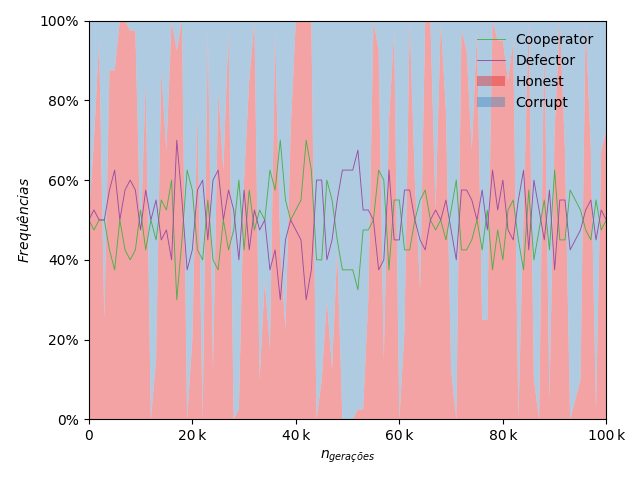
\includegraphics[width=1\linewidth]{images/AggregateComparison.png}
        \caption{\small Dinâmica das estratégias dos árbitros e resultado da aprendizagem social racional. $b=1, c=0.5, f=B=0.2, h=0.1, A=2, M=40, N=40, \mu=0.001, \nu=0.001, \beta=1000$}
        \label{fig:ciclos_agregados}
    \end{figure}

    Nas figuras \ref{fig:ciclos_agregados} e \ref{fig:ciclos} conseguimos distinguir a presença de ciclos nas estratégias dos árbitros e consoante a intensidade de selecção, ciclos ou convergência nas estratégias dos jogadores. Quando a intensidade de seleção é muito alta ou muito baixa, os agentes são respectivamente racionais ou aleatórios e verifica-se ciclicidade nas frequências das estratégias.

    Na figura \ref{fig:ciclos} observamos que quando existe maior abundância de árbitros corruptos na população os jogadores desertores florescem enquanto os jogadores cooperadores diminuiem. Por sua vez, quando os árbitros honestos abundam, os desertores tendem a diminuir, o que corresponde aos resultados esperados e intuitivos.

    \begin{figure}[h]
        \centering
        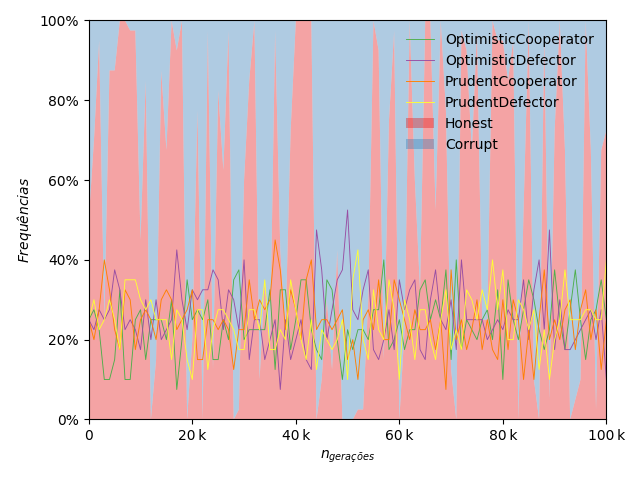
\includegraphics[width=1\linewidth]{images/Comparison.png}
        \caption{\small Impacto da qualidade da regulação nas estratégias dos agentes racionais. $b=1, c=0.5, f=B=0.2, h=0.1, A=2, M=40, N=40, \mu=0.001, \nu=0.001, \beta=1000$}
        \label{fig:ciclos}
    \end{figure}
    Estes ciclos são explicados pela dinâmica que existe entra as duas populações: Quando existem muitos árbitros corruptos, as estratégias mais vantagosas são as dos desertores que conseguem subornar o árbitros e recebem um payoff maior, mas com maior número de corruptos os cooperadores prudentes deixam de jogar e o payoff dos árbitros corrutos deixa de ser vantagoso e passam a haver mais árbitros honestos. Com o aparecimento de mais árbitros honestos também há um aumento de cooperadores otimistas, que confiam no árbitro sem precisar de saber à priori se ele é ou não honesto. Com este comportamento dos cooperadores, os desertores e os árbitros corruptos voltam a aparecer outra vez. \\

    \section{Small mutation limit}
    Nesta secção estudaremos o problema sobre uma perpetiva um pouco mais matemática recorrendo ao estudo de processos estocásticos e fazendo várias aproximações.\\
    Vamos assumir que a probabilidade de mutação é muito pequena (no limite é quase 0) e portanto se tivermos uma população de jogadores inteiramente formada por jogadores de uma única estratégia, como a probabilidade de mutação é muito pequena podemos assumir que a probabilidade de ocorrerem várias mutações ao mesmo tempo é nula. Ou seja, se uma mutação ocorrer numa população monomórfica (apenas com uma única estratégia) só teremos de calcular a probabilidade de fixação \cite{2} da estratégia mutante, isto é,a probabilidade de toda a população adotar a estratégia escolhida aleatóriamente com a probabilidade $\mu$ para o caso dos jogadores e $\nu$ para o caso dos árbitros. Para simplificar aqui vamos considerar que $\mu=\nu$.

    Assim, no limite, vamos ter os oito estados monómorficos que podem transitar de uns para os outros segundo o simplex seguinte que representa uma cadeia de markov:

    \begin{figure}[h]
        \centering
        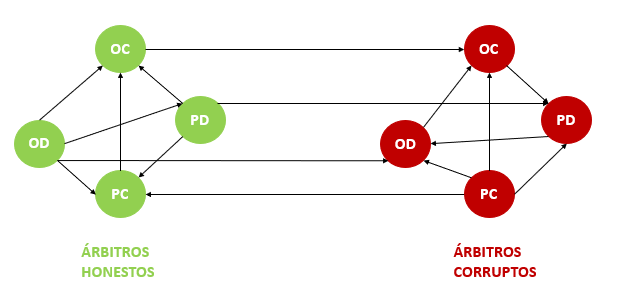
\includegraphics[width=1\linewidth]{images/GRAFO.PNG}
        \caption{\small Representação da cadeia de Markov dos oito estados. cada estado é um estado monomórfico ou seja nas duas populações só há uma única estratégia. Por exemplo o Estado OC com árbitros honestos é um estado onde todos os jogadores são cooperadores otimistas e todos os árbitros são honestos}
    \end{figure}
    É de notar que neste cenário, como a probabilidade de mutação é muito pequena nas duas populações, mutações simultaneas nas duas populações não vão ser consideradas, ou seja, a probabilidade de fixação de um estado para outro, onde as duas populações (tanto dos jogadores como dos árbitros ) se alterem, vai ser sempre 0. (Por exemplo ir do estado OD com árbitro honesto para o estado PC com o árbitro corrupto).\\

    Construindo o fitness de cada estratégia conseguimos calcular as probabilidades de fixação da seguinte forma:
    $\\$
    \begin{center}
        $p_{ab}=\sum_{i=0}^{N-1}\prod_{j=1}^{i}\frac{T^{-}(j)}{T^{+}(j)}$\\
        $\\$
    \end{center}

    onde $p_{ij}$ é a probabilidade de fixação do estado $b$ estando no estado $a$. $T^{+}$ é a probabilidade do número de mutantes aumentar em um, analogamente $T^{-}$ é a probabilidade do número de mutantes decrescer em um\\
    $\\$
    $T^{+}$ e $T^{-}$ são dados por:\\

    $T^{+}=\frac{j-1}{N}\frac{N-j}{N-1}{(1+e^{-beta(fit(a,b,j,ump,0)-fit(a,b, j,ump,1))})}^{-1}$\\
    e \\

    $T^{-}=\frac{j-1}{N}\frac{N-j}{N-1}{(1+e^{beta(fit(a,b,j,ump,0)-fit(a,b,j,ump,1))})}^{-1}$\\

    onde $fit(a, b, j, ump, 0)$ representa o fitness da estratégia mutante a, havendo j mutantes da estratégia a na população, N-j jogadores da estratégia b e com todos os umpires com a mesma estratégia (ump = honesto ou ump=corrupto), e o $fit(a,b,j, ump, 1)$ representa o fitness da estratégia b havendo j mutantes de a.

    calculando todas as probabilidades de fixação conseguimos calcular a matriz de transição da cadeia de markov, onde cada entrada tem a probabilidade de fixação dividida pelo numero de estados menos 1 (neste caso sete).

    Para facilitar os cálculos, consideramos que as duas populações têm o mesmo tamanho ou seja M=N.

    Na figura \ref{fig:primeira} é apresentado uma matriz de transição e a respetiva distribuição estacionária. Podemos notar que os estados onde o árbitro é corrupto são os estados onde a cadeia passa mais tempo.
    Com esta abordagem podemos facilmente perceber quais os estados mais vesitados ou seja quais as estratégias mais usadas.

    \begin{figure}[h]
        \centering
        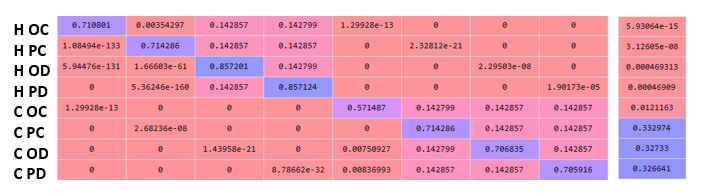
\includegraphics[width=1\linewidth]{images/PRIMEIRA.PNG}
        \caption{\small Matriz de transição e respetiva distribuição estacionária dos vários estados. Parametros utilizados: M=N=40, $\beta=2, f=0.2, b=0.1, c=0.5, h=0.1, B=0.2,A=2, \mu=\nu$ }
        \label{fig:primeira}
    \end{figure}

    \newpage

    \section{Resultados Adicionais}
    Até agora tentámos recriar os resultados apresentados por Lee e Iwasa em \cite{1} chegando às mesmas conclusões onde temos ciclos endémicos de corrupção na população. No entanto não foram consideradas algumas variações ao modelo que podem ter impacto nos resultados descritos acima. O nosso objetivo passa por tentar quebrar o ciclo de corrupção com a ligeira alteração ao modelo original.
    Assim, nesta secção alteramos o modelo inicial de duas formas e vemos como estas variações atuam e alteram a dinâmica das duas populações.
    Nestas variações continuamos a utilizar as simulações numéricas e a técnica do small mutation limit para conseguirmos olhar para o problema de duas perpetivas diferentes.

    \subsection{Incerteza nas informações recebidas por jogadores prudentes}
    Uma das variações ao modelo que é interessante considerar é ver como a dinâmica muda se considerarmos que a informação obtida pelos jogadores prudentes acerca dos árbitros não for $100\%$  fidedigna.\\
    No modelo inicial, um jogador prudente que paga um custo $h$ receberá a informação correta acerca da estratégia do árbitro sem nenhuma incerteza relativamente à validade da informação. Aqui, consideramos que essa informação poderá estar certa com probabilidade $p$ ou errada com probabilidade $1-p$. Esta incerteza faz com que jogadores prudentes, que à partida podiam não entrar num jogo devido à estratégia do árbitro (jogadores PC não jogam com árbitros corruptos e jogadores PD não jogam com árbitros honestos), recebam a informação errada acabando por participar no jogo. Esta variação altera os payoffos tanto dos jogadores como dos árbitros (que podem ser consultados na secção \ref{Anexos}).\\

    Para conseguirmos medir o impacto desta medida, fizemos as simulações utilizando os mesmos valores para todos os parametros iniciais, e só modificamos $p$ que inicialmente correspondia a 100\%. Testamos o caso onde $p=0.75$, $p=0.5$ e $p=0.0$.
    \\

    \begin{figure}[h]
        \centering
        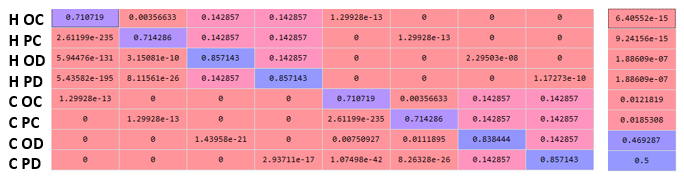
\includegraphics[width=1\linewidth]{images/SEGUNDA_P_0_5.PNG}
        \caption{\small Matriz de transição e respetiva distribuição estacionária dos vários estados. Parametros utilizados: $M=N=40, \beta=2, f=0.2, b=0.1, c=0.5, h=0.1, B=0.2,A=2, \mu=\nu, p=0.5$}
        \label{fig:segunda}
    \end{figure}

    \begin{figure}[h]
        \centering
        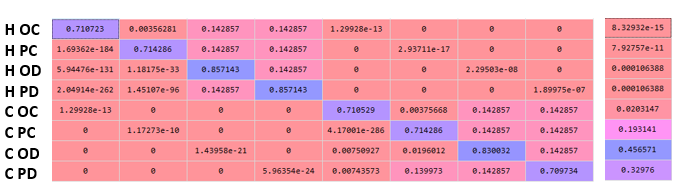
\includegraphics[width=1\linewidth]{images/terceira_0_75.PNG}
        \caption{\small Matriz de transição e respetiva distribuição estacionária dos vários estados. Parametros utilizados: $M=N=40, \beta=2, f=0.2, b=0.1, c=0.5, h=0.1, B=0.2,A=2, \mu=\nu, p=0.75$ }
        \label{fig:terceira}
    \end{figure}

    Analisando os resultados é notório que à medida que a probabilidade dos jogadores obterem informações fidedignas sobre o árbitro diminui, os desertores vão ser claramente beneficiados, principalmente os desertores optimistas, conforme podemos ver no cenário presente na figura \ref{fig:incerteza_total}. O jogo torna-se mais vantagoso para árbitros corruptos e por conseguinte para jogadores desertores - o que não é completamente intuitivo. Esta conclusão pode também ser tirada das distribuições estacionárias dado que para $p=50\%$ os estados mais vesitados são os estados dos árbitros corruptos e os jogadores são desertores.

    \begin{figure}[h]
        \centering
        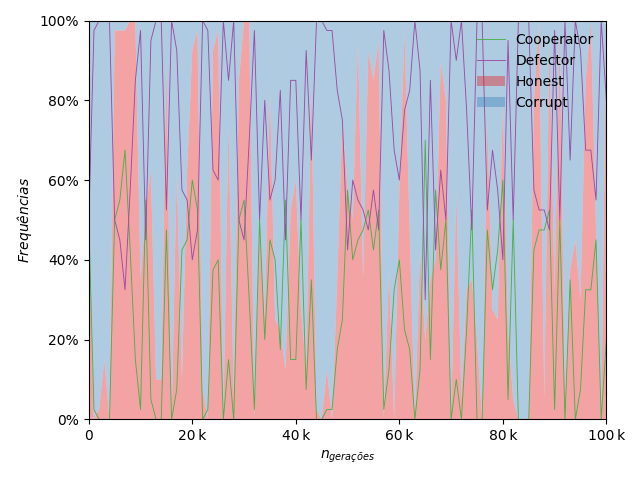
\includegraphics[width=1\linewidth]{images/incerteza_total.png}
        \caption{\small Informações erradas beneficiam árbitros desonestos e jogadores desertores. $b=1, c=0.5, f=B=0.2, h=0.1, A=2, M=40, N=40, \mu=0.001, \nu=0.001, \beta=10^{10}, p=0$}
        \label{fig:incerteza_total}
    \end{figure}

    \subsection{Punição de árbitros}
    Outra questão que pode fazer diferença é ver como a ecologia dos árbitros e jogadores se altera com a introdução de uma punição aos árbitros desonestos. No modelo original os jogadores que são desertores podem ser punidos pelos árbitros, no entanto, não há nenhuma punição para árbitros corruptos. Tradicionalmente este papel é desempenhado pelo poder judicial mas neste caso apenas iremos considerar a punição em si e não a emergência de um novo tipo de agente que pune os árbitros.\\
    Neste caso vamos considerar que os árbitros são sempre punidos com um custo T quando agem como corruptos (quando há pelo menos um desertor a jogar e o árbitro aceita o suborno) ou quando um jogador prudente sabe que ele é corrupto. \\ Assim a matriz dos payoffs dos árbitros corruptos é alterada para:

    \begin{table}[h]
        \centering
        \begin{tabular}{c|cccc}
            Estratégias&OC&PC&OD&PD\\
            \hline
            OC & 2f & -T & 2f+B-T & 2f+B-T\\
            PC & -T & -T & -T & -T\\
            OD & 2f+B-T & -T & 2(f+B)-T & 2(f+B)-T\\
            PD & 2f+B-T & -T & 2(f+B)-T & 2(f+B)-T\\
        \end{tabular}
        \caption{Payoffs dos árbitros corruptos}
    \end{table}
    \\
    Aqui, tal como na secção anterior, nas simulações fixámos os valores dos parâmtros do modelo inicial e fizemos variar o valor da punição dos árbitros T.
    Tanto com as simulações numéricas como com o uso do small mutation limit, podemos ver que esta medida faz com que um maior predominância de árbitros honestos na população, no entanto, os ciclos, continuam a verificar-se. \\  É ainda de reparar que mesmo com a queda dos árbitros corruptos, na distribuição estacionária podemos ver que os estados mais prováveis são os desertores. Podemos ainda dizer que se o valor da punição do árbitro for menor que o valor do suborno , $T<B$ , então a queda da quantidade de corruptos não é tão acentuada.


    \begin{figure}[h]
        \centering
        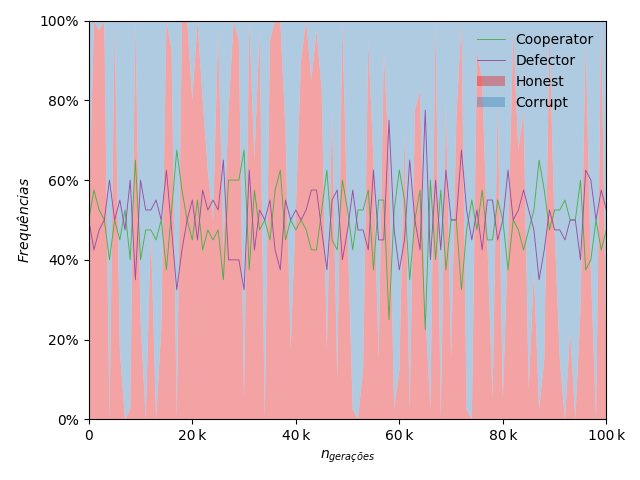
\includegraphics[width=1\linewidth]{images/punishment.png}
        \caption{\small A introdução de mecanismos de punição aumenta a prevalência de árbitros honestos. $b=1, c=0.5, f=B=0.2, h=0.1, A=2, M=40, N=40, \mu=0.001, \nu=0.001, \beta=10^{10}$}
        \label{fig:punicao}
    \end{figure}

    \begin{figure}[h]
        \centering
        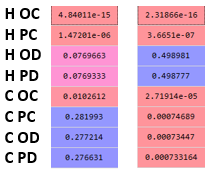
\includegraphics[width=0.5\linewidth]{images/T'S_FIN.PNG}
        \caption{\small Matriz de transição e respetiva distribuição estacionária dos vários estados. Parametros utilizados: M=N=40, $\beta=2$, f=0.2, b=0.1, c=0.5, h=0.1, B=0.2,A=2, $\mu=\nu$ T=0.1 para a figura da esquerda e T=0.3 para a figura da direita. Notamos que para T=0.3 os árbitros corruptos são quaase inexistentes para a distribuição limte. }
    \end{figure}

    \section{Apontamentos finais}
    Neste trabalho analisámos duas variações do modelo inicial, sempre com o objetivo de tentar quebrar o ciclo. Isto foi conseguido com a punição de árbitros corruptos, no entanto, na prática esta pode não ser a melhor estratégia para que a corrupção não tenha valores elevados. Aqui, deixamos algumas sugestões de medidas que poderiam travar o ciclo de corrupção e aumentar a cooperação entre jogadores.

    \begin{itemize}
        \begin{enumerate}
            \item  Para além de punir os árbitros corruptos com um custo T, premiar, com o mesmo valor, os jogadores cooperadores que fossem prejudicados com a corrupção.
            \item Criar uma nova população, com o intuito de punir os árbitros, onde os membros dessa população pudessem jogar como desertores ficticios e sempre que um árbitro corrupto fosse subornado por um destes elementos, o árbitro era de alguma forma punido.
        \end{enumerate}
    \end{itemize}

    Este caso ainda pode ser estudado com mais detalhe fazendo uma análise criteriosa da variação dos parâmetros. Todavia com uma análise superficial, conseguimos dizer que a corrupção da forma como foi formulada tem um caráter ciclico, no entanto pode ser quebrado quando não só os jogadores desertores como os árbitros corruptos são punidos. E ainda que a informação errada contribui para agravar a situação da corrupção.

    \bibliographystyle{plain}
    \bibliography{bib}

    \onecolumn

    \section{Anexos} \label{Anexos}
    \begin{table}[h]
        \centering
        \begin{tabular}{c|cccc}
            Estratégias&OC&PC&OD&PD\\
            \hline
            OC & b-c-f & p(b-c-f)          & -c-f & (1-p)(-c-f)\\
            PC & p(b-c-f-h)-(1-p)h & p(b-c-f-h)-(1-p)h & p(-c-f-h)-(1-p)h & -h\\
            OD & b-f-A & p(b-f-A)          & -f-A & (1-p)(-f-A)\\
            PD & -ph+(1-p)(b-f-A-h) & -h & -ph+(1-p)(-f-A-h) & -ph+(1-p)(-f-A-h)\\
        \end{tabular}
        \caption{Payoffs dos jogadores com árbitro honesto com incerteza na informação à priori sobre o árbitro}
    \end{table}

    \begin{table}[h]
        \centering
        \begin{tabular}{c|cccc}
            Estratégias&OC&PC&OD&PD\\
            \hline
            OC & b-c-f & (1-p)(b-c-f)       & -c-f & p(-c-f)\\
            PC & -ph+(1-p)(b-c-f-h)   & -ph+(1-p)(b-c-f-h) & -ph+(1-p)(-c-f-h)   & -h\\
            OD & b-f-B & (1-p)(b-f-B)       & -f-B & p(-f-B)\\
            PD & p(b-f-B-h)+(1-p)(-h) & -h & p(-f-B-h)+(1-p)(-h) & p(-f-B-h)+(1-p)(-h)\\
        \end{tabular}
        \caption{Payoffs dos jogadores com árbitro corrupto com incerteza na informação à priori sobre o árbitro}
    \end{table}

    \begin{table}[h]
        \centering
        \begin{tabular}{c|cccc}
            Estratégias&OC&PC&OD&PD\\
            \hline
            OC & 2f & 2pf & 2f & 2(1-p)f\\
            PC & 2pf & 2pf & 2pf & 0\\
            OD & 2f & 2pf & 2f & 2(1-p)f\\
            PD & 2(1-p)f & 0 & 2(1-p)f & 2(1-p)f\\
        \end{tabular}
        \caption{Payoffs dos árbitros honestos}
    \end{table}

    \begin{table}[h]
        \centering
        \begin{tabular}{c|cccc}
            Estratégias&OC &PC &OD &PD\\
            \hline
            OC & 2f & 2(1-p)f & 2f+B & 2pf+pB\\
            PC & 2(1-p)f & 2(1-p)f & 2(1-p)f+(1-p)B & 0\\
            OD & 2f+B & 2(1-p)f+(1-p)B & 2f+2B & 2p(f+B)\\
            PD & 2pf+pB & 0 & 2p(f+B)         & 2p(f+B)\\
        \end{tabular}
        \caption{Payoffs dos árbitros corruptos}
    \end{table}

\end{document}